% !TEX root = B&G_oefeningen.tex
\chapter{Binaire zoekbomen (BST)}


\section*{Inleiding}

Download het bestand \verb=week03_BST_opgave.zip= van Toledo en importeer dit bestand in IntelliJ zoals aangegeven in de oefeningen van vorige week. 

\begin{oef}
\papier Gegeven twee binaire bomen in figuren~\ref{fig:BSToef1} en \ref{fig:oefBST2}. Ga voor elk van beide na of het een binaire zoekboom is (BST).
\begin{figure}[htbp]
    \centering
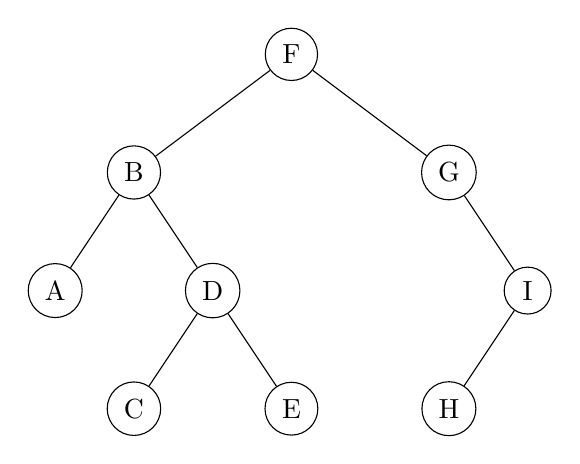
\begin{tikzpicture}[every node/.style={circle,draw},
				level 1/.style={sibling distance=40mm},
				level 2/.style={sibling distance=20mm}]
\node {F}
child { node {B} 
	child { node {A} }
	child { node {D} 
		child { node {C} } 
		child { node {E} } }
}
child { node {G}
	child[missing]
	child { node {I}
		child { node {H}}
		child[missing]}};
\end{tikzpicture}
\caption{Een binaire boom, maar is het ook een BST?}
    \label{fig:BSToef1}
\end{figure}

\begin{figure}[htbp]
    \centering
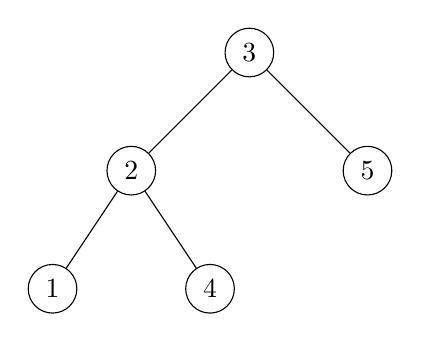
\begin{tikzpicture}[every node/.style={circle,draw},
				level 1/.style={sibling distance=30mm},
				level 2/.style={sibling distance=20mm}]
\node {3}
child { node {2} 
	child { node {1} }
	child { node {4} }
}
child { node {5}};
\end{tikzpicture}
\caption{Een binare boom met getallen in de knopen}
    \label{fig:oefBST2}
\end{figure}

\begin{opl}
De eerste boom (figuur~\ref{fig:BSToef1}) is een BST omdat elke knoop (alfabetisch) groter is dan alle knopen in de linkersubboom en kleiner dan alle knopen in de rechtersubboom. De tweede boom (figuur~\ref{fig:oefBST2}) is echter geen BST omdat 3 niet groter is dan 4 (terwijl de knoop 4 toch in de linkersubboom zit).
\end{opl}
\end{oef}



\newpage
\begin{oef}
\papier Kan je een BST doorlopen met 1 van de 3 strategie\"en besproken in les 3 (pre-order, in-order of post-order) zodanig dat de knopen worden bezocht van klein naar groot?
\begin{opl}
We bekijken nog eens de definitie van binaire zoekboom: voor elke knoop in de boom geldt dat zijn waarde strikt groter is dan alle waarden in zijn linkersubboom en strikt kleiner dan alle waarden in zijn rechtersubboom. Deze volgorde is ook wat een in-order doorloop doet.
\end{opl}
\end{oef}





\begin{oef}
\papier In deze oefening krijg je een vaste structuur waar je de datavelden moet invullen.
\begin{oefenumerate}
\item Op hoeveel verschillende manieren kan je de getallen 3 tot en met 9 in onderstaande knopen invullen met als resultaat een BST?  Teken deze verschillende mogelijkheden.
\begin{figure}[htbp]
    \centering
\begin{tikzpicture}[every node/.style={circle,draw},
			level 1/.style={sibling distance=30mm},
			level 2/.style={sibling distance=15mm},]
\node {\phantom{7}}
child { node {\phantom{5}} 
	child { node {\phantom{4}} 
		child { node {\phantom{3}}}
		child[missing]}
	child { node {\phantom{6}} }
	}
child { node {\phantom{9}}
	child { node {\phantom{8}}}
	child[missing]
	};
\end{tikzpicture}
\caption{Getallen van 3 t.e.m. 9 invullen in de knopen}
    \label{fig:oefBST39}
\end{figure}

\item Kan je de getallen 3 tot en met 9 opslaan in een andere BST waarvoor de worst-case tijdscomplexiteit van de \verb=lookup= methode kleiner is? Zo ja, geef deze BST. Zo nee, leg uit waarom niet.
\end{oefenumerate}


\begin{opl}
Er is maar één mogelijke oplossing, nl. figuur~\ref{fig:oefBST39opl}.
\begin{figure}[htbp]
    \centering
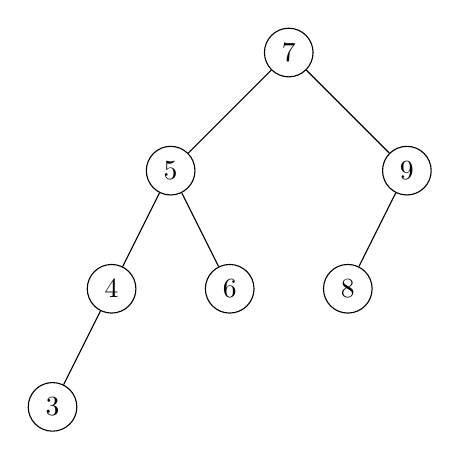
\begin{tikzpicture}[every node/.style={circle,draw},
			level 1/.style={sibling distance=30mm},
			level 2/.style={sibling distance=15mm},]
\node {7}
child { node {5} 
	child { node {4 } 
		child { node {3}}
		child[missing]}
	child { node {6} }
	}
child { node {9}
	child { node {8}}
	child[missing]
	};
\end{tikzpicture}
\caption{Getallen van 3 t.e.m. 9 invullen in de knopen}
    \label{fig:oefBST39opl}
\end{figure}
\end{opl}
\end{oef}






\begin{oef}
\papier \code Bestudeer de klasse \verb=BinarySearchTree= en de \verb=BinaryTree= in de package (\verb=domain=) in de \verb=src= folder.
 Een eerste  methode is \verb=lookUp= waarmee snel een bepaalde waarde in de BST kan opgezocht worden (zie de slides van deze les). Een tweede methode is \verb=addNode= waarmee gegeven data aan de BST kan toegevoegd worden.

\begin{oefenumerate}
\item Teken op papier eerst de binaire zoekboom zoals die door de \verb+main+ methode in de klasse \verb+BinarySearchTreeDriver+ zal worden toegevoegd.
\item Implementeer de \verb=addNode= methode in de \verb=BinaryTree= klasse.  Maak optimaal gebruik van het feit dat de boom een binaire zoekboom is.
\item Om je implementatie te controleren, run je de BinarySearchTreeDriver klasse uit de \verb+ui+ package. Verwachte uitvoer: 3 4 5 6 7 8 9  
\end{oefenumerate}
\begin{opl}
De \verb+main+ methode construeert de (gebalanceerde) BST uit figuur~\ref{fig:oefBSTmain}.
\begin{figure}[htbp]
    \centering
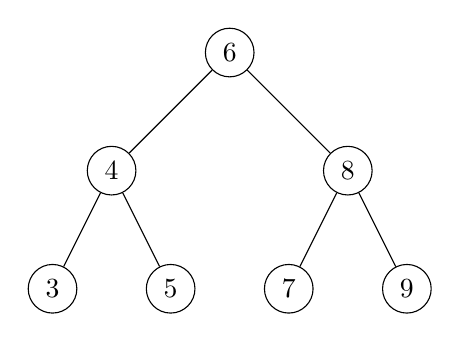
\begin{tikzpicture}[every node/.style={circle,draw},
			level 1/.style={sibling distance=30mm},
			level 2/.style={sibling distance=15mm},]
\node {6}
child { node {4} 
	child { node {3}}
	child { node {5}}
	}
child { node {8}
	child { node {7}}
	child { node {9}}
	};
\end{tikzpicture}
\cprotect\caption{ResultaatBST van de \verb+main+ methode}
    \label{fig:oefBSTmain}
\end{figure}
\begin{lstlisting}[caption={addNode(data) methode}, label=bstaddnode]
public boolean addNode(E data) {
	if (data == null) {
		throw new IllegalArgumentException();
	}
	if (this.data.compareTo(data) == 0) {
		return false; //geen twee keer zelfde data in BST
	} else if (this.data.compareTo(data) > 0) {//ga naar linkersubboom
		if (this.leftTree == null) {
			this.leftTree = new BinarySearchTree<>(data);
			return true;
		} else return (this.leftTree.addNode(data));
	} else if (this.rightTree == null) {
		this.rightTree = new BinarySearchTree<>(data);
		return true;
	} else return (this.rightTree.addNode(data));
}
\end{lstlisting}

\end{opl}
\end{oef}


\begin{oef}
\code Implementeer nu ook de methode \verb=lookUp= in de \verb=BinaryTree= klasse en controleer je implementatie door in de BinarySearchTreeDriver-klasse een aantal knopen op te zoeken. Maak een efficiënte implementatie die de voordelen van een binaire zoekboom benut. Zoek ook een niet bestaande knoop op.
\begin{opl}
\begin{lstlisting}[caption={lookUp(data) methode}, label=bstlookUp]
public boolean lookup(E data) {
	if (data == null) {
		return false;
	}
	if (this.data.compareTo(data) == 0) {
		return true;
	} else {
		if (this.data.compareTo(data) > 0) {
			return (this.leftTree == null ? false : this.leftTree.lookup(data));
		} else {
			return (this.rightTree == null ? false : this.rightTree.lookup(data));
		}
	}
}
\end{lstlisting}
\end{opl}
	
\end{oef}





\begin{oef}
\code Het doel van deze oefening is een implementatie te maken van een methode die de grootste waarde uit de BST teruggeeft.
\begin{oefenumerate}
	\item Implementeer de \verb=searchGreatest= methode in de \verb=BinaryTree= klasse. 
	\item Om je implementatie te controleren, run je de BinarySearchTreeDriver klasse uit de \verb+ui+ package. Verwachte uitvoer: De grootste waarde uit deze boom = 9 
\end{oefenumerate}
\begin{opl}
\begin{lstlisting}[caption={searchGreatest methode}, label=bstsearchgreatest]
public E searchGreatest() {
	if (this.rightTree == null) {
		return this.data;
	} else {
		return this.rightTree.searchGreatest();
	}
}
 \end{lstlisting}

\end{opl}
\end{oef}




\begin{oef}
\code Programmeer een methode die de kleinste waarde uit de BST teruggeeft.
\begin{oefenumerate}
	\item Implementeer de \verb=searchSmallest= methode in de \verb=BinaryTree= klasse.  
	\item Om je implementatie te controleren, run je de BinarySearchTreeDriver klasse uit de \verb+ui+ package. Verwachte uitvoer: De kleinste waarde uit deze boom = 3
\end{oefenumerate}
\begin{opl}
\begin{lstlisting}[caption={searchSmallest methode}, label=bstsearchsmallest]
public E searchSmallest() {
	if (this.leftTree == null) {
		return this.data;
	} else {
		return this.leftTree.searchSmallest();
	}
}
\end{lstlisting}
\end{opl}
\end{oef}



\begin{oef}
\code \emph{Deze en de volgende oefening beschouwen we niet als leerstof. Ze staan hier voor studenten die een extra uitdaging zoeken. Je moet het verwijderen van een node wel kennen voor het schriftelijk examen, maar hoeft het dus niet te kunnen programmeren.}

Een volgende methode is \verb=removeNode= waarmee gegeven data uit de BST zal verwijderd worden indien mogelijk. 
\begin{oefenumerate}
\item Implementeer de \verb=removeNode= methode in de \verb=BinarySearchTree= klasse. 
\item Om je implementatie te controleren, kan je de klasse  \verb=BinarySearchTreeDriver= aanpassen en uit de opgebouwde BST uit oefening 4 de knoop met dataveld 9 te verwijderen.

	
	
\end{oefenumerate}
\begin{opl}
%Figuur~\ref{fig:oefBSTuitgebreid} toont de uitgebreide BST
%\begin{figure}[htbp]
%    \centering
%\begin{tikzpicture}[every node/.style={circle,draw},
%			level 1/.style={sibling distance=30mm},
%			level 2/.style={sibling distance=15mm},]
%\node {6}
%child { node {4} 
%	child { node {3}}
%	child { node {5}}
%	}
%child { node {8}
%	child { node {7}}
%	child { node {9}
%		child[missing]
%		child { node {10}
%			child[missing]
%			child { node {11}}
%			}
%		}
%	};
%\end{tikzpicture}
%\cprotect\caption{BST uitgebreid met de getallen 10 en 11}
%    \label{fig:oefBSTuitgebreid}
%\end{figure}
\begin{lstlisting}[caption={removeNode methode}, label=bstremovenode]
public boolean removeNode(E data) {
	if (data == null) {
		throw new IllegalArgumentException();
	}
	if (this.data == null) {
		return false;
	}
	if (this.data.compareTo(data) == 0) {//data gevonden
		if (this.isLeaf()) {
			this.data = null;
			return true;
			// in dit geval blijft een leeg blaadje achter
			// clean kan dan enkel via gehele boom
		} else {
			if (this.leftTree != null) {//linkerboom is niet leeg
				E grootsteLinks = this.leftTree.searchGreatest();
				this.data = grootsteLinks;
				boolean verwijderenGelukt = this.leftTree.removeNode(grootsteLinks);
				if (verwijderenGelukt) {
					this.leftTree.cleanUp();
				}
				return verwijderenGelukt;
			} else {//rechterboom is niet leeg
				E kleinsteRechts = this.rightTree.searchGreatest();
				this.data = kleinsteRechts;
				boolean verwijderenGelukt = this.rightTree.removeNode(kleinsteRechts);
				if (verwijderenGelukt) {
					this.rightTree.cleanUp();
				}
				return verwijderenGelukt;
			}
		}
	} else {
		if (this.data.compareTo(data) > 0) {//zoek in linkerboom
			return (this.leftTree == null ? false : this.leftTree.removeNode(data));
		} else {//zoek in rechterboom
			return (this.rightTree == null ? false : this.rightTree.removeNode(data));
		}
	}
}
\end{lstlisting}

\end{opl}
\end{oef}




\begin{oef}
\papier \code Een probleem dat weggesnoeid moet worden …
\begin{oefenumerate}
\item Implementeer de \verb=countNodes= methode in de \verb=BinarySearchTree= klasse die het aantal knopen in een boom telt. Na de verwijdering van de knoop met data-veld 9 valt iets eigenaardigs op: het verwijderen van de knoop heeft geen effect op het aantal knopen. We onderzoeken dat in de volgende deelvragen.
	\item Teken  de boom die je na het verwijderen van de knoop met waarde 9 kreeg. Eén van de bladeren van de boom heeft nu als data de waarde \verb+null+ gekregen.
	\item Blaadjes met als datawaarde \verb+null+ laten we niet aan de boom staan. Tijd om te snoeien! Schrijf een methode \verb+cleanUp()+ die deze ‘verdorde’ blaadjes verwijdert. Pas ze toe op de boom na het verwijderen van de knoop met waarde 9 en laat zien dat het aantal knopen na de snoeibeurt wel degelijk ééntje verminderd is.  
	\item Voeg nog twee knopen toe aan de BST uit oefening 4 met data-velden 10 en 11. Schrijf de boom uit na een in-order wandeling (verwachte uitvoer: 3,4,5,6,7,8,9,10,11). Verwijder tenslotte uit deze boom data-veld 9, data-veld 11 en data-veld 6 en ruim lege blaadjes op. De verwachte uitvoer van een in-order wandeling is dan: 3 4 5 7 8 10.
\end{oefenumerate}
\begin{opl}
\begin{lstlisting}[caption={ruimOp methode}, label=bstruimop]
private void cleanUp() {
	if (this.data != null) {
		if (this.leftTree != null) {
			if (this.leftTree.data == null) {
				this.leftTree = null;
			} else {
				this.leftTree.cleanUp();
			}
		}
		if (this.rightTree != null) {
			if (this.rightTree.data == null) {
				this.rightTree = null;
			} else {
				this.rightTree.cleanUp();
			}
		}
	}
}
\end{lstlisting}
\end{opl}

\end{oef}


\begin{oef}
\code In deze oefening schrijf je een methode die gegeven een data-veld een pad teruggeeft van de wortel van de boom tot het dataveld indien mogelijk. We passen dit toe op de boom die je als resultaat na vorige oefening zou moeten bekomen. Bij wijze van controle: figuur~\ref{fig:oefgetpathboom} toont deze boom met zes knopen.
\begin{figure}[htbp]
    \centering
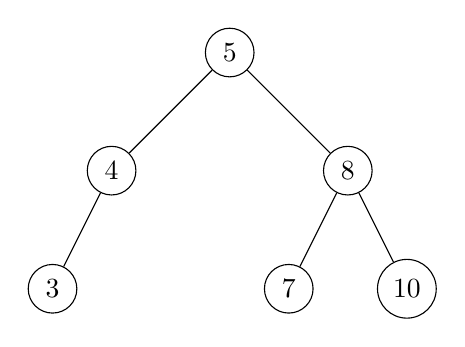
\begin{tikzpicture}[every node/.style={circle,draw},
			level 1/.style={sibling distance=30mm},
			level 2/.style={sibling distance=15mm},]
\node {5}
child { node {4} 
	child { node {3}}
	child[missing]
	}
child { node {8}
	child { node {7}}
	child { node {10}}
	};
\end{tikzpicture}
\cprotect\caption{BST na uitbreiding met knopen 10 en 11 en verwijdering van 9, 11 en 6}
    \label{fig:oefgetpathboom}
\end{figure}
\begin{oefenumerate}
	\item Implementeer de \verb=getPath= methode in de \verb=BinarySearchTree= klasse. 
	\item Als controle pas je de klasse  \verb=BinarySearchTreeDriver= aan zodat je drie keer de methode \verb+getPath+ oproept met als parameter respectievelijk 7, 4 en 8. De uitvoer moet dan respectievelijk zijn: bij 7: [5,8,7] ; bij 4: [5, 4] en bij 8: [5, 8]. Probeer de methode ook uit met als parameter 22. In dit geval moet de methode \verb+null+ als returnwaarde hebben.
	
\end{oefenumerate}
\begin{opl}
\begin{lstlisting}[caption={getPath methode}, label=bstgetpath]
public ArrayList<E> getPath(E data) {
	if (!lookup(data)) {//data komt niet voor in BST
		return null;
	}
	ArrayList<E> pad = new ArrayList<>();
	if (this.data.compareTo(data) == 0){
		pad.add(data);
		return pad;
	} else {
		pad.add(this.data);
		if (this.data.compareTo(data) > 0) {//ga links, data komt zeker voor!
			pad.addAll(this.leftTree.getPath(data));
		} else {// ga rechts, data zit daar gegarandeerd
			pad.addAll((this.rightTree.getPath(data)));
		}
	}
	return pad;
}
\end{lstlisting}

\end{opl}
\end{oef}

\begin{oef}
\papier Neem de boom van figuur~\ref{fig:BSToef1}. Teken achtereenvolgens de boom als je eerst knoop G verwijdert, dan knoop B en tenslotte knoop F.
\begin{opl}
Zie figuren \ref{fig:G}, \ref{fig:GB} en \ref{fig:GBF}.
\begin{figure}[H]
    \centering
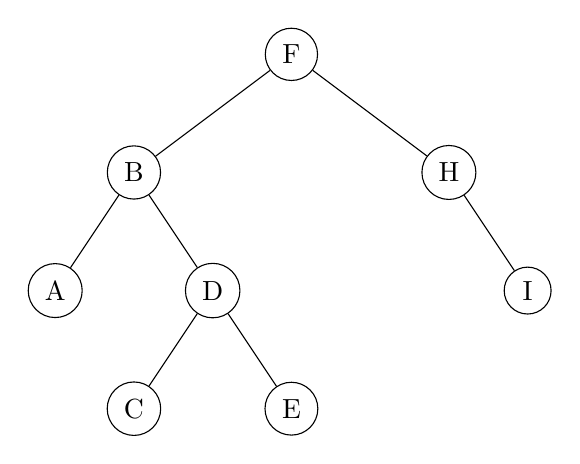
\begin{tikzpicture}[every node/.style={circle,draw},
				level 1/.style={sibling distance=40mm},
				level 2/.style={sibling distance=20mm}]
\node {F}
child { node {B} 
	child { node {A} }
	child { node {D} 
		child { node {C} } 
		child { node {E} } }
}
child { node {H}
	child[missing]
	child { node {I}}};
\end{tikzpicture}
\caption{Boom \ref{fig:BSToef1} na verwijderen van knoop G}
\label{fig:G}
\end{figure}

\begin{figure}[H]
    \centering
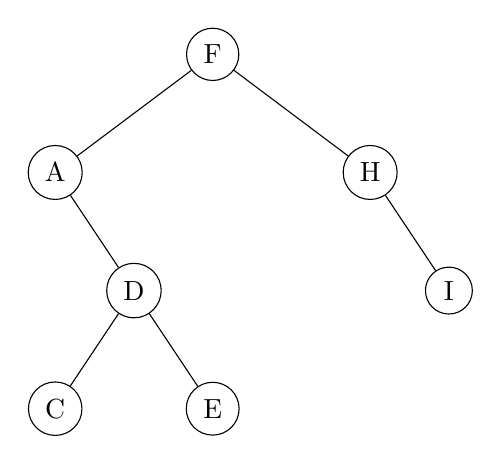
\begin{tikzpicture}[every node/.style={circle,draw},
				level 1/.style={sibling distance=40mm},
				level 2/.style={sibling distance=20mm}]
\node {F}
child { node {A} 
	child[missing]
	child { node {D} 
		child { node {C} } 
		child { node {E} } }
}
child { node {H}
	child[missing]
	child { node {I}}};
\end{tikzpicture}
\caption{Boom \ref{fig:BSToef1} na verwijderen van knoop G en B}
\label{fig:GB}
\end{figure}

\begin{figure}[H]
    \centering
\begin{tikzpicture}[every node/.style={circle,draw},
				level 1/.style={sibling distance=40mm},
				level 2/.style={sibling distance=20mm}]
\node {E}
child { node {A} 
	child[missing]
	child { node {D} 
		child { node {C} } 
		child[missing] } 
}
child { node {H}
	child[missing]
	child { node {I}}};
\end{tikzpicture}
\caption{Boom \ref{fig:BSToef1} na verwijderen van knoop G, B en F}
\label{fig:GBF}
\end{figure}


\end{opl}
\end{oef}






